% Created 2024-11-30 Sat 21:43
% Intended LaTeX compiler: pdflatex
\documentclass[11pt]{article}
\input{../../../preamble.tex}

% setting up title page
\title{
  
\includegraphics[width=0.4\textwidth]{fmf_logo}\\
  {\small Oddelek za fiziko} \\
  {Sunkovna jedrska magnetna resonanca}\\
  {\small Poročilo pri FP5}\\

}
\date{}
\author{ Kristofer Č. Povšič, 28211104 \\[5 cm]
 \small  Asistent: Tilen Knaflič \\
}
\addbibresource{refs.bib}

\begin{document}

\maketitle
\newpage
\tableofcontents
\newpage

\section{Uvod}\label{sec:orgf006394}

Jedro ima poleg vrtilne količine \(\vec{\Gamma}\) tudi magnetni moment \(\vec{\mu}\). Vrtilna količina in magnetni moment imata isto smer in sta povezana z enačbo

\begin{equation}
\label{eq:1}
\vec{\mu} = \gamma \vec{\Gamma}
\end{equation}

kjer je \(\gamma\) giromagnetno razmerje, ki je odvisno od vrste jedra.

V magnetnem polju \(\vec{B}_0\), ki naj kaže vzdolž osi \(z\), deluje na magnetni moment navor

\begin{equation}
\label{eq:2}
\vec{N} = \vec{\mu} \times \vec{B}_0 = \gamma \vec{\Gamma} \times \vec{B}_0
\end{equation}

Sprememba vrtilna količine je sorazmerna sunku navora, kar da enačbo

\begin{equation}
\label{eq:3}
\frac{\mathrm{d} \vec{\Gamma}}{\mathrm{dt}} = \vec{N} = \gamma \vec{\Gamma} \times \vec{B}_0
\end{equation}

Sprememba vrtilne količine je vedno pravokotna na sunek in na magnetno polje. Iz tega sledi, da magnetni moment precesira okoli smeri magnetnega polja z Larmorjevo frekvenco

\begin{equation}
\label{eq:4}
\omega_L = \gamma \left| \vec{B}_0 \right|
\end{equation}

Če v homogeno magnetno polje postavimo snov, ki ima neničelna jedra s spinom \(\vec{\Gamma}\) in magnetnim momentom \(\vec{\mu}\) se v njej pojavi magnetizacija, ki je magnetni moment na enoto volumna.

Tudi ta precesira okrog smeri magnetnega polja z Larmorjevo frekvenco, kadar ni vzporedna z njim.

Imamo še dodatno magnetno polje \(\vec{B}_1\), ki kaže v smeri \(x\), pravokotno na smer statičnega polja, in oscilira z Larmorjevo frekvenco. Za kratek čas vključimo \(\vec{B}_1\) in kot med magnetizacijo in statičnim magnetnim poljem \(\vec{B}_0\) se poveča.

Velikost kota je odvisna od amplitude in časa trajanja polja \(\vec{B}_1\). Posebej zanimivi so sunki, ki spremenijo kot za \(\pi\) ali \(\frac{\pi}{2}\).

Dodatno magnetno polje povzročimo s tuljavico, ki je napajana s sunkovnim radiofrekvenčnim (RF) izvorom električnega izvora. Tako govorimo o sunkih \(\pi\) in \(\frac{\pi}{2}\).

Definiramo vrteči se sistem znotraj laboratorijskega, ki se vrti okoli smeri magnetnega polja z Larmorjevo frekvenco \(\omega_L\):

\begin{align*}
  z ' &= z \\
x' &= x \cos \left( \omega_L t \right) + y \sin \left( \omega_L t \right) \\
y' &= y \cos \left( \omega_L t \right) - x \sin \left( \omega_L t \right)
\end{align*}

Dodatno magnetno polje tako zapišemo kot

\[ \vec{B}_1 = B_1 (\cos \left( \omega_L t \right), 0, 0)
\]

Prva komponenta se vrti skupaj z vrtečim se sistemom, ki smo ga definirali in je v njem statična vzdolž osi \(x'\). Z vpeljavo vrtečega polja smo upoštevali statično magnetno polje \(\vec{B}_0\). To pomeni, da magnetizacija \(\vec{M}\) precesira okoli osi \(x'\) in ne več okoli \(z\). Edino, kar je, je to, da se magnetizacija odkloni za nek kot od \(z = z'\).

Sunek \(\frac{\pi}{2}\) obrne polarizacijo v smer osi \(y'\) in ne čuti nobenega zunanjega magnetnega polja. Ker je magnetizacija vsota magnetnih momentov posameznih jeder, ne ostane obrnjena vzdolž osi \(y'\), ampak se s časom vrne v termodinamsko ravnovesno vrednost.

Projekcije magnetnim momentov se v ravnini \(x'y'\) prej povrnejo v ravnovesno stanje (aka raztresenost), kakor pa se njihova komponenta \(z'\). Projekcija magnetizacije na ravnino \(x'y'\) zato eksponento pada z razpadno konstanto \(T_2\), ki jo imenujemo spinsko-spinski relaksacijski čas.

Na čas \(T_2\) vpliva samo interakcija med magnetnimi momenti, zato tudi tako ime.

Poleg izgube fazne povezave se zmanjšuje tudi azimut posameznega magnetnega momenta. Projekcija na os \(z'\) se zato povečuje s karakterističnim časom \(T_1\), ki ga imenujemo tudi spinsko-mrežni relaksacijski čas

\begin{equation}
\label{eq:6}
M_{z'} = M(1 - e^{-\frac{t}{T_1}})
\end{equation}

Če imamo nehomogeno magnetno polje, projekcija magnetizacije v ravnino \(x'y'\) ne pada več eksponento s časom \(T_2\), ampak kot neka druga krivulja \(T_2^{*}\), ki je odvisna od \(T_2\), nehomogenosti magnetnega polja in od oblike vzorca.

Ocenimo ga lahko kot
\begin{equation}
\label{eq:5}
T_2^{*} \approx \frac{\pi}{2} \frac{1}{\gamma \Delta B_z} \approx \frac{1}{\gamma \Delta B_z}
\end{equation}

Po sunku \(\frac{\pi}{2}\) je magnetni moment obrnjen v smeri osi \(y'\) in nato precesira okoli osi \(z'\) z neko frekvenco \(\omega\). V času \(\tau\) se zavrti za kot \(\phi = \omega \tau\) glede na os \(y'\). S sunkom \(\pi\) se magnetni moment zasuka v nasprotno smer \(\pi - \omega \tau\). Po času \(2\tau\) bodo magnetni momenti ponovno v smeri osi \(-y'\), saj je \(\phi(2\tau) = \pi - \omega \tau + \omega \tau\).

V merilni tuljavici se zato pojavi signal, ki ga imenujemo spinski odmev. Amplituda spinskega odmeva z večanjem razmaka med sunkoma pada kot

\[ e ^{-\frac{2\tau}{T_2}}
\]

širina pa je odvisna od tega, kako hitro se magnetni momenti spet zberejo nazaj v smeri \(-y'\) in je enaka \(T_2^{*}\).
\section{Potrebščine}\label{sec:org02fc6c0}

\begin{itemize}
\item NMR spektrometer
\item vzorci vode
\item osciloskop
\item napajalnik
\item vodno hlajenje
\item elektromagnet
\end{itemize}
\section{Naloge}\label{sec:org4d45467}

\begin{itemize}
\item za vzorec vode s primešanimi paramagnetnimi ioni poišči signal proste precesije po sunku \(\frac{\pi}{2}\) in signal spinskega odmeva po zaporedju sunkov \(\frac{\pi}{2}\) in \(\pi\). Z opazovanjem širine proste precesije in signala spinskega odmeva poišči takšno lego sonde, da bo magnetno polje v področju vzorca čimbolj homogeno. Iz obeh širin izračunaj \(T_2^{*}\) in oceni nehomogenost magnetnega polja v vzorcu
\item Z opazovanjem odvisnost signala proste precesije med dvema sunkoma \(\frac{\pi}{2}\) določi relaksacijski čas \(T_1\) za vzorec vode s primešanimi paramagnetnimi ioni in za vzorec vodovodne vode
\item Za vodo s primešanimi paramagnetnimi ioni poišči odvisnost višine signala spinskega odmeva od presledka \(\tau\) med sunkoma \(\frac{\pi}{2}\) in \(\pi\) in določi spinsko-spinski relaksacijski čas \(T_2\).
\end{itemize}

\section{Meritve in obdelava podatkov}\label{sec:org93542d4}
Vse .csv datoteke sem obdelal v programerskem jeziku Python z njegovimi knjižnicami numpy, matplotlib, pandas, scipy, uncertainties in cmasher.
\subsection{Ocena \(T_2^{*}\) in nehomogenosti polja}\label{sec:org135c7a5}
Vzorec vode s paramagnetnimi ioni sem postavil v magnet in iz širine grafov na slikah \ref{fig:prosta_procesija} in \ref{fig:spinski_odmev} ocenil vrednost konstante \(T_2^{*}\).

\begin{figure}[H]
  \centering
  \begin{minipage}[b]{0.4\textwidth}
    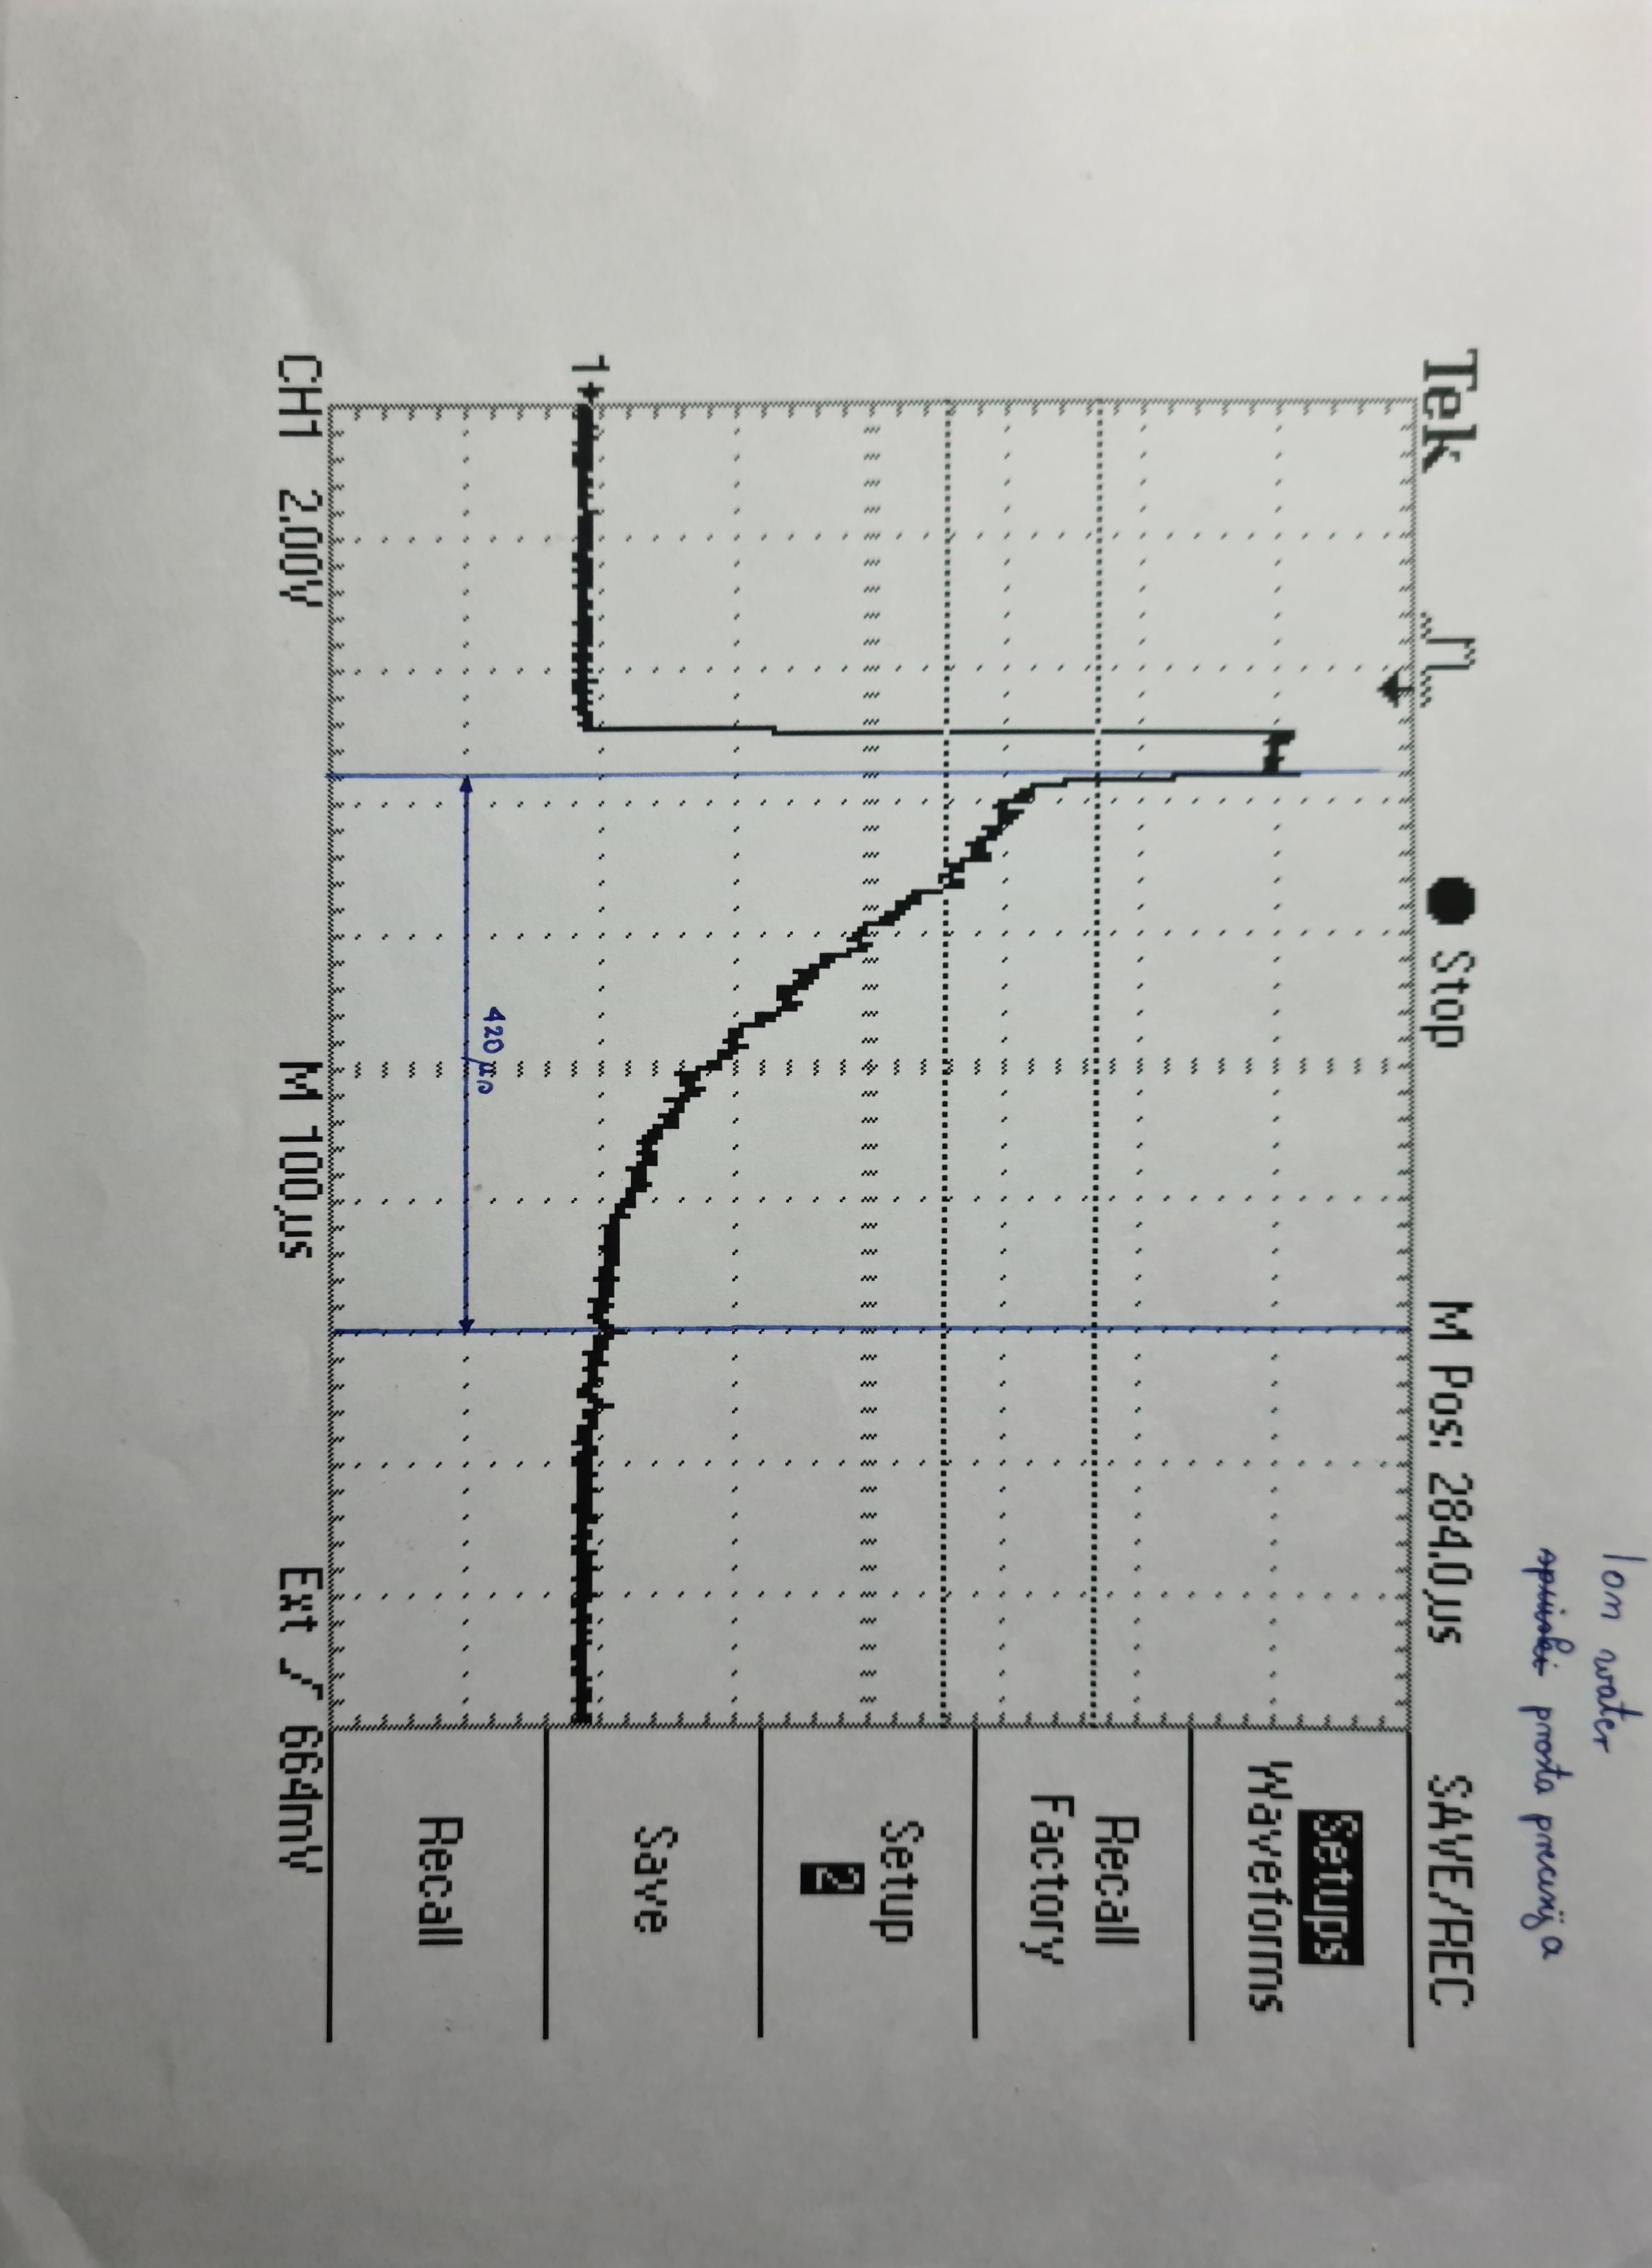
\includegraphics[width=\textwidth]{figures/20241129_153343.jpg}
    \captionof{slika}{\small Slika prikazuje graf signala proste precesije zajet na osciloskopu.}\label{fig:prosta_procesija}
  \end{minipage}
  \hfill
  \begin{minipage}[b]{0.4\textwidth}
    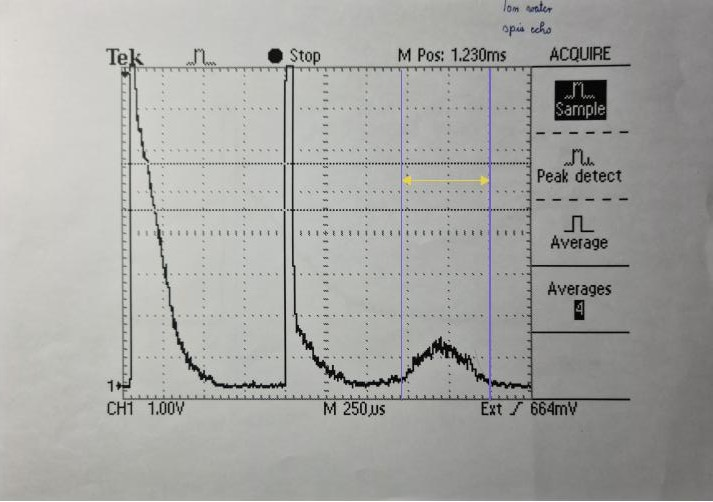
\includegraphics[width=\textwidth]{figures/spinski_odmev.jpg}
     \captionof{slika}{\small Slka prikazuje graf signala spinskega odmeva in odčitane vrednosti za ocenitev \(  T_{2}^{*} \)}\label{fig:spinski_odmev}
  \end{minipage}
\end{figure}
Graf proste precesije sem uvozil v WebPlotDigitizer (vir \cite{webplotdigitizer}), ročno poklikal točke in jih izvozil v .csv datoteko.

Podatke sem potem logaritmiral in jih regresiral premici na grafu \ref{fig:t2_zvezdica} ter dobil oceno

\[ T_2^{*} \doteq (0.269 \pm 0.04 ) \mathrm{ms}
\]
\begin{slika}[H]
\begin{center}
  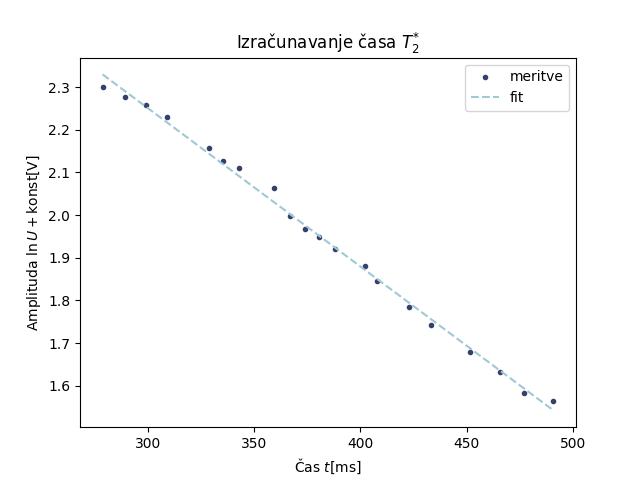
\includegraphics[width=.9\linewidth]{figures/cas_t2_zvezdica.png}
  \caption{\small Graf prikazuje regresivno premico ter podatke odčitane iz grafa \ref{fig:prosta_procesija} preko \cite{webplotdigitizer}.}\label{fig:t2_zvezdica}
\end{center}
\end{slika}


Iz grafa spinskega odmeva \ref{fig:spinski_odmev} lahko prav tako ocenimo relaksacijski čas, saj je odmev širok \(2 \cdot T_2^{*}\).

\[ T_2^{*} \doteq 0.26 \mathrm{ms}
\]

Iz danih podatkov lahko sedaj po enačbi \ref{eq:5} ocenimo nehomogenost magnetnega polja, ki je enaka

\[ \Delta B_z \doteq (1.39 \pm 0.02) \mu \mathrm{T}
\]
\subsection{Umeritev časovne skale}\label{sec:orgd2f454d}

Premik gumba na NMR spektrometru ni popolnoma enak časovni enoti na osciloskopu, zato je bilo potrebno to tudi umeriti. Narisal sem graf in iz točk regresiral premico, katere vrednost sem potem uporabljal v nadaljnem obdelovanju podatkov.

\begin{slika}[H]
\begin{center}
  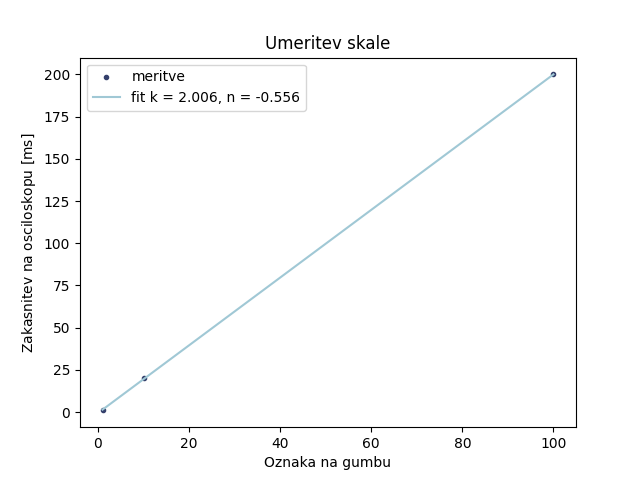
\includegraphics[width=.9\linewidth]{figures/umeritev_skale.png}
  \caption{\small Graf prikazuje umeritev gumbov na NMR spektrometru. }\label{fig:umeritev}
\end{center}
\end{slika}

\subsection{Spinsko-mrežni relaksacijski čas \(T_1\)}\label{sec:org45f3957}
Izmerjene podatke za vodo z in brez paramagnetnih ionov sem regresiral sem enačbo \ref{eq:6}. Grafa se lahko vidi na \ref{fig:t1_ion} in \ref{fig:t1_tap}.

\begin{slika}[H]
\begin{center}
  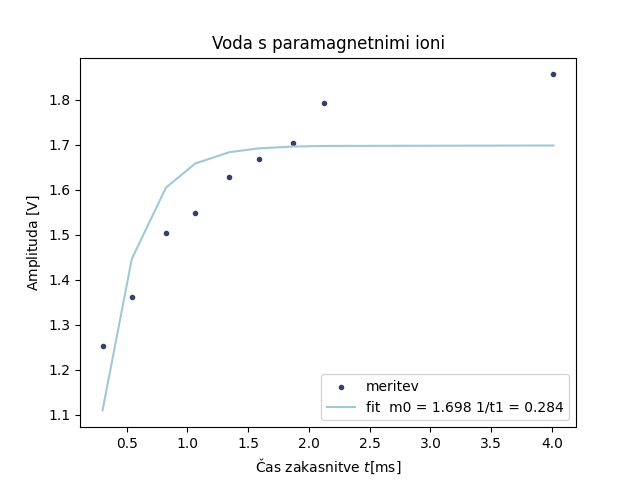
\includegraphics[width=.9\linewidth]{figures/t1_ion.png}
  \caption{\small Graf prikazuje regresije eksponentne funkcije \ref{eq:6} na izmerjene podatke vode s paramagnetnimi ioni. Računali smo spinsko-mrežni relaksacijski čas \( T_{1} \).}\label{fig:t1_ion}
\end{center}
\end{slika}

\begin{slika}[H]
\begin{center}
  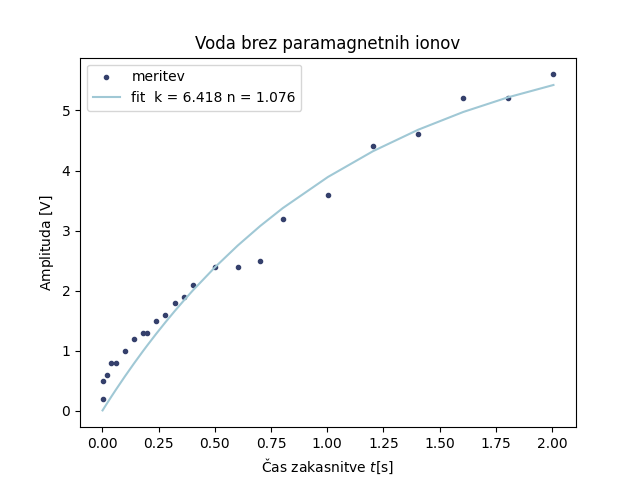
\includegraphics[width=.9\linewidth]{figures/t1_tap.png}
  \caption{\small Graf prikazuje regresije eksponentne funkcije \ref{eq:6} na izmerjene podatke vode brez paramagnetnih ionov. Računali smo spinsko-mrežni relaksacijski čas \(  T_{1  } \)}\label{fig:t1_tap}
\end{center}
\end{slika}

Dobil sem sledeči vrednosti

\begin{align*}
  T_{1 ion} &= (3.5 \pm 0.6) ms \\
T_{1 tap} &= (0.15 \pm 0.01) s
\end{align*}

\subsection{Spinsko-spinski relaksacijski čas \(T_2\)}\label{sec:orgefcfe41}
Z logaritmirano meritvijo signala spinskega odmeva v odvisnosti od razmika \(\tau\) med sunkoma \(\frac{\pi}{2}\) in \(\pi\) lahko s prileganjem premice določimo čas \(T_2\) za vodo s primešanimi ioni. Za vodovodno vodo je ta čas predolg in tako smo iz grafa \ref{fig:spinski_t2} dobili

\begin{slika}[H]
\begin{center}
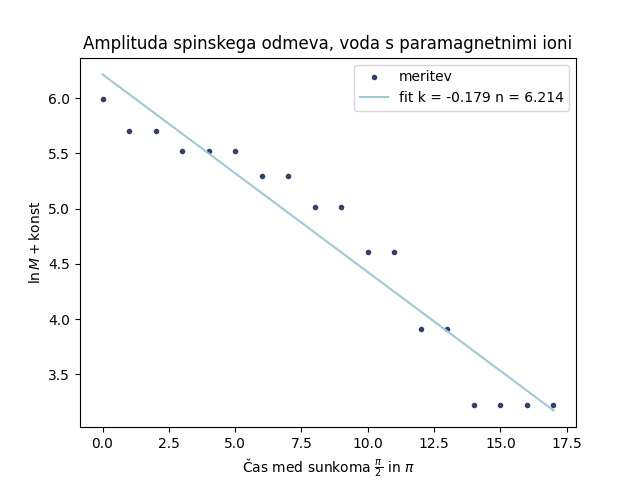
\includegraphics[width=.9\linewidth]{figures/spinski_odmev_t2.png}
\caption{\small Graf prikazuje odvisnost logaritmiranega signala spinskega odmeva od odvisnosti razmika \(  \tau \). }\label{fig:spinski_t2}
\end{center}
\end{slika}

in vrednost

\[ T_2 = 5.6 \pm 0.4 ms
\]
\section{Komentar}\label{sec:org50e2e3d}

Pri oceni časa \(T_2^{*}\) sem moral uporabiti logaritmirane podatke, saj je imela funkcija curve\_fit težave najti prave vrednosti parametrov za eksponentno funkcijo. Ocena relaksacijskih časov iz spinskega odmeva ter proste precesije se precej dobro ujemata.

Tako pri umeritvi časovne skale kot pri spinsko-mrežno relaksacijskem času \(T_1\) za vodo s paramagnetnimi ioni bi ob ponovitvi vaje, želel opraviti večje število meritev. Že pri danih podatkih je regresirana funkcija za čas \(T_1\) izjemno slaba. Medtem ko se pri vodovodni vodi precej bolje ujema.

Kot je pisalo v navodilih je je krivulja \(T_2^{*}\) samo podobna krivulji \(T_2\), kar razloži neujemanje vrednosti. Bi pa rekel, da je nekega smiselnega velikostnega reda.
\printbibliography[heading=bibintoc]
\end{document}
